\section{Anonymous communication systems}

Why are VPNs and TLS not enough? VPN server still sees metadata such as srcIP, dstIP, ports, metadata etc. We need something stronger for anonymous communication. TLS does not hide src and dest address.

\subsection{Terminology: “anonymity”}

\begin{itemize}
	\item \textbf{Sender anonymity:} adversary knows/is receiver, may learn message, sender is unknown. The sender anonymity set is the set of all possible senders, which can be used as a (rough) metric. A small set means little anonymity. Return address is a token provided by original sender.
	\item \textbf{Receiver anonymity:} Adversary knows sender, may learn message, receiver is unknown. The sender needs a return address: the receiver provides a token (since the sender doesn't know the receiver) and the token will be used to direct the message. Receiver anonymity set is the set of all possible receivers.
	\item \textbf{(Sender-receiver) unlinkability:} Adversary knows senders, knows receivers, link between senders and	receivers is unknown. Multiple users need to communicate at the same time. Anonymity --> Unlinkability
	\item \textbf{Unobservability:} Adversary cannot tell whether any communication is taking place.
	\item \textbf{Plausible Deniability:} Adversary cannot prove that any particular individual was responsible for a message (or other action). Anonymity --> plausible deniability
\end{itemize}

The following holds: $Unobservability \rightarrow Anonymity \rightarrow Unlinkability$

\paragraph{Threat Model: } 
\begin{itemize}
    \item Degree of control: Local or global
    \item Type of Control: network or compromised infrastructure
    \item Types of Behavior: passive or active
    \item Often quite unspecified attacker model --> unclear guarantees
\end{itemize}

\subsection{Basics of Anonymous Communication}

\paragraph{What Mechanisms can we use?}
\begin{itemize}
    \item \textbf{Broadcast:} Receiver anonymity is guaranteed, sender can be de-anonymized (localization through triangulation)!. 
    \item \textbf{Hijacked Connection:} burner phone, hacked WiFi, network ID != personal sender ID.
    \item \textbf{Proxy or VPN with layered encryption:} Proxy can see metadata (src, dest) 
    \item[-->] \textbf{Cascade of multiple proxies} Each proxy only sees addresses of two neighbors, due to layered encryption. Works as long as message passes one honest proxy. 
    \item[-->] However the attacker may link in and outgoing messages through timing.
\end{itemize}

\subsection{Mixnets}

\paragraph{Batching and Mixing:}
Collect a number of messages before forwarding (Batching), change the order of the messages (Mixing), also we need to padd messages to a fixed length.\\
An adversary can still mount an \textbf{intersection attack:} Often, users only communicate with a
small subset of other users. Every time a message is seen by the target, register the sets of destinations. 

\paragraph{Cover traffic for unobservability:}
To achieve full unobservability, use \textbf{cover traffic}, both for sending and receiving. Now we are fully anonymous, as long as one mix is honest. \\
How do we handle return addresses? Alice prepares a return address and encloses it in her first message. That address contains layered information.


\subsection{Circuit-based systems (AKA onion-routing system)}
Mix-nets are very secure but very slow. We want a system that can support web browsing.\\
Circuit-based anonymous communication systems, commonly known as Onion Routing Systems. The nodes are called relays (also nodes or routers), there are usually 3 of them Entry guard, Middle relay and Exit relay. The virtual circuit is also called tunnel.
\begin{itemize}
    \item Main ideas: use layered encryption, no batching and mixing, no cover traffic.
    \item Flow-based: establish a virtual circuit (keys) once per flow, reuse it for all packets in the flow using only symmetric key crypto.
    \item The threat model is constrained: only a local adversary (e.g. ISP) which cannot launch confirmation attacks.
\end{itemize}

\paragraph{Circuit setup}
\begin{itemize}
    \item Initially, sender knows long-term public keys of relays.
    \item The sender negotiates shared keys with all relays on the path (this requires expensive asymmetric key cryptography)
    \item The relays store the necessary state.
\end{itemize}
\textbf{Direct circuit setup:} a packet is sent through the whole system and returned and at each step the state is generated. The encryption keys of data are only based on public keys of relays. Thus (immediate) Forward Security does not hold since no ephemeral information is used. We can achieve eventual forward security by changing public keys of the relays regularly \\
\textbf{Telescopic circuit setup:} Keys are negotiated one relay at a time. The circuit is “extended” by one hop at a time (that’s why it is called telescopic). Ephemeral session keys are negotiated before the circuit is extended. This setup is slower... but it offers immediate forward secrecy: As soon as the circuit is closed, the session keys are deleted.

\paragraph{Data forwarding}

The sender has established a circuit (keys and per-link IDs). A data packet is encrypted as usual (layered encryption). The ID of the next relay is added in clear text. To protect against network adversaries, links can be encrypted (TLS).

\paragraph{Circuit tear-down}

Can be initiated both by sender and by intermediate relays. The sender communicates the tear-down to one relay at a time, starting from the furthest away. The exit relay may tear down the circuit if a corrupt packet is detected, or some other attack. Circuits have a limited lifetime, so they will eventually be destroyed.

\begin{minipage}{\linewidth}
    \centering      
    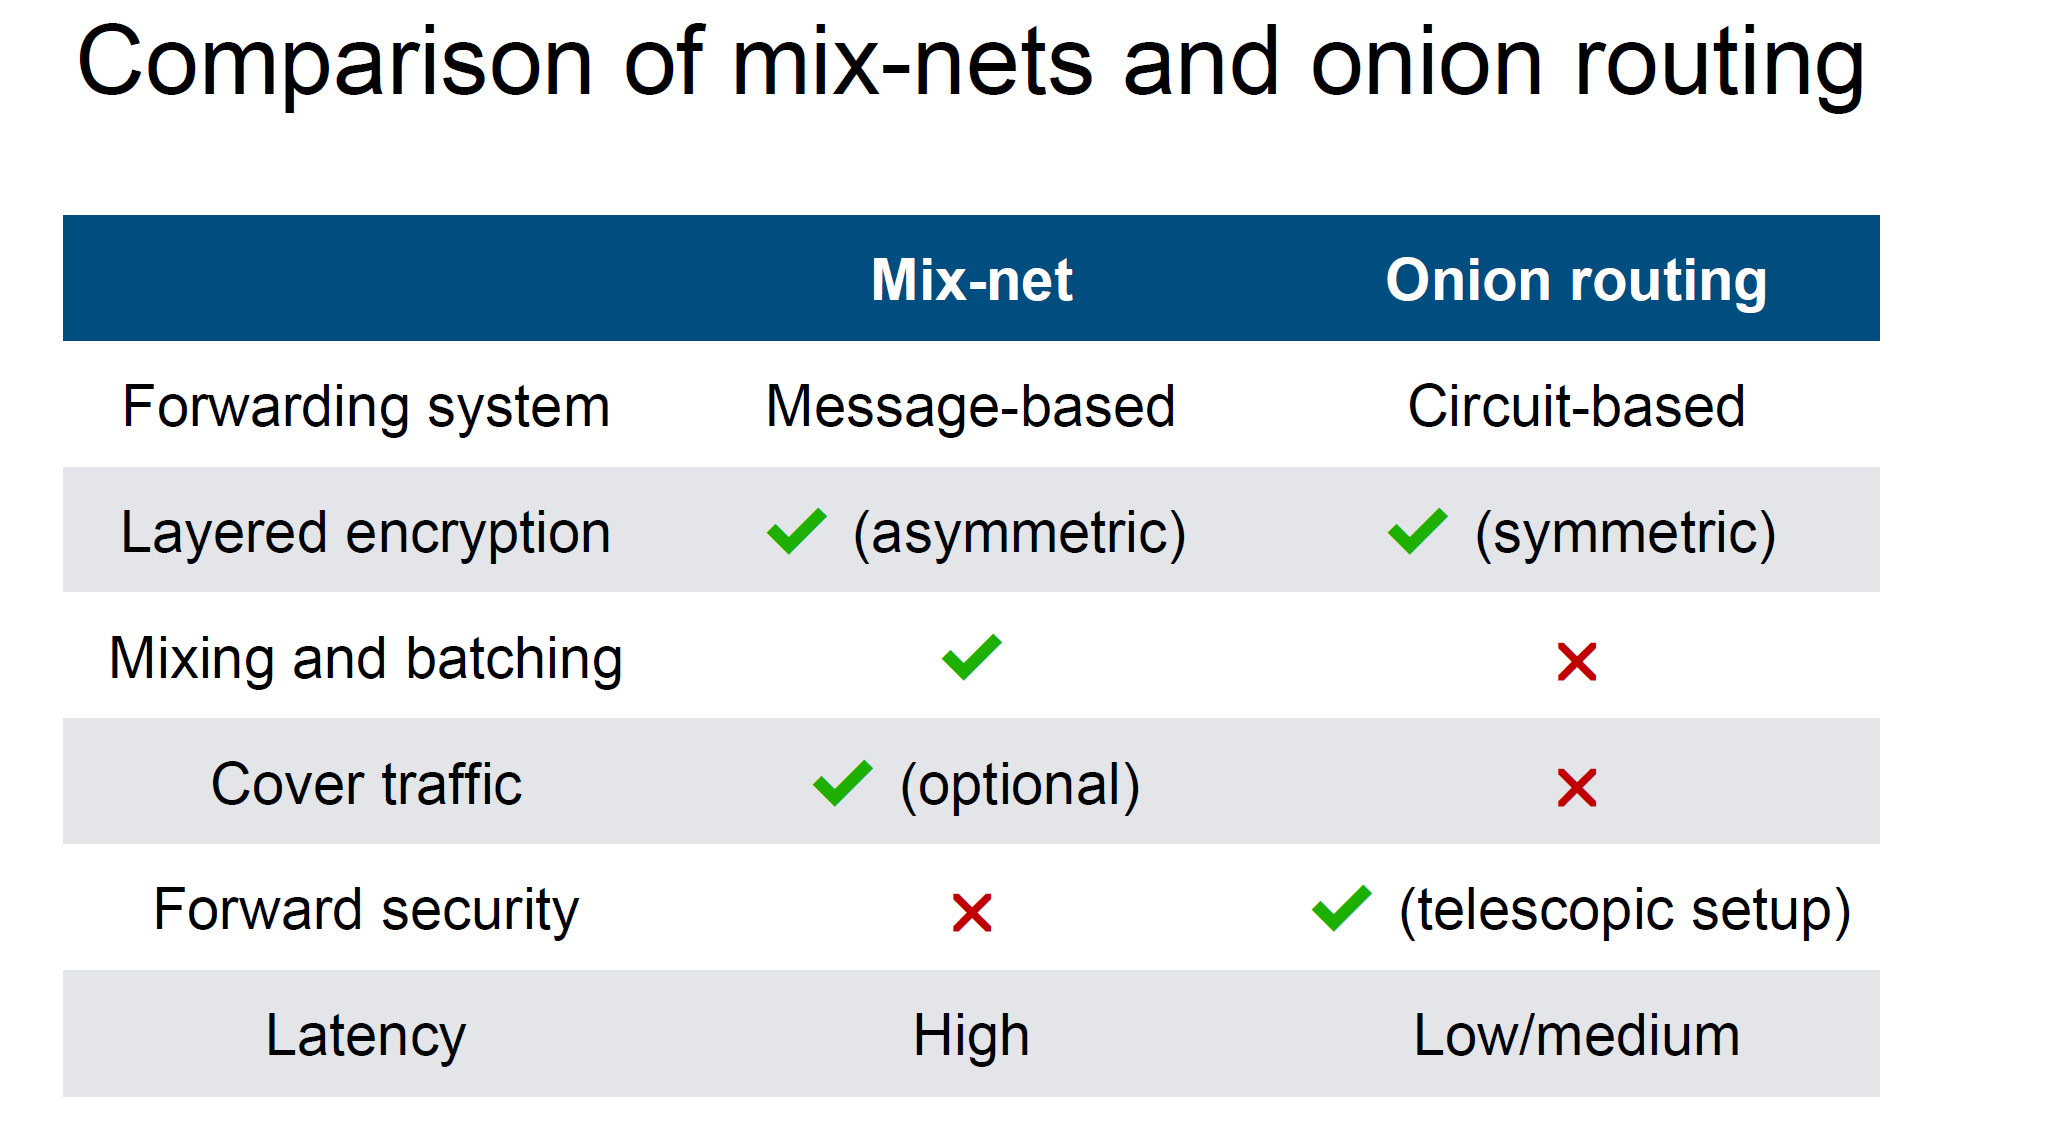
\includegraphics[width=\linewidth]{Figures/Anym_mix_nets.PNG} 
\end{minipage}

\subsection{Attacks on circuit-based anonymous-communication systems}

Many attacks have been proposed, however for many it is unclear if they fit the standard threat model. Some of them are practical, requiring limited resources. Others are only achievable by state-level adversaries (Five Eyes).

\paragraph{Traffic Analysis:}
\begin{itemize}
	\item Passive traffic analysis: The adversary observes the edges of the network, recording traffic patterns. Real-time detection is challenging, alternative is store and compare later.
	\item Active traffic analysis: 
	\begin{itemize}
		\item The adversary actively modifies packet timings: Inter-packet timings (delaying/reordering packets), packet drops also possible but detectable
		\item Flow watermarking: inject one bit of information (marked or not)
		\item Flow fingerprinting: inject multiple bits (e.g., sender IP address!)
	\end{itemize}
	\item Website fingerprinting: Many websites have a distinct pattern of traffic they receive and send. Adversary can keep a database of patterns and compare traffic recorded from a single observation point (ISP, WiFi users,...)
\end{itemize}

\paragraph{Denfence against Traffic Analysis:}
\begin{itemize}
    \item Cover traffic and mixing: significant overhead, scalability becomes an issue. Only suitable for few applications (VoIP) with low bandwidth.
\end{itemize}

In order to prevent traffic analysis, you should omit \textit{everything} that makes you stand out: don't install any plugins, never use TOR in fullscreen mode (gives away your screen resolution), don't type inside the browser, type inside a text-editor and copy-paste messages into webforms, etc.

\subsubsection{Higher-layer attacks}
\begin{itemize}
	\item OS Network stack fingerprinting: Compromised adversary can probe TCP stack, solution would be per-hop TCP. Still TLS or HTTP layer may be identifiable.
	\item Most deanonymization is still done through other means: Trick user into downloading malware, trick user into downloading file that will access the Internet directly, analyze user behavior like texts.
\end{itemize}

To achieve anonymity, all layers need to be anonymized: Any gap will break anonymity!

\subsection{Tor}

\paragraph{Tor basics:}
\begin{itemize}
	\item Circuits established over 3 relays
	\item Telescopic setup (forward secrecy!)
	\item Per-hop TCP, established on the fly to avoid TCP stack fingerprinting
	\item Per-hop TLS (except on the last hop). Multiple circuits over same TLS connection. End-to-end HTTPS is possible.
	\item Main tool: Tor browser (Firefox)
\end{itemize}

\paragraph{Tor additional features:}

\begin{itemize}
	\item Exit policies (exit can restrict the destinations	they connect to)
	\item Multiple streams per circuit (helps with performance, weakens anonymity)
	\item Censorship resistance (bridges)
	\item Hidden services: Provide receiver anonymity, use .onion URL (not in DNS). The name is the hash of the HS’s public key.
\end{itemize}

\subsubsection{Cells}

Basic unit in Tor. If a relay obtains a cell: it looks up keying material from circuit id and will decrypt the payload which contains sets of fields. The relay then checks the digest and if it matches it looks at the cmd.

\begin{minipage}{\linewidth}
    \centering      
    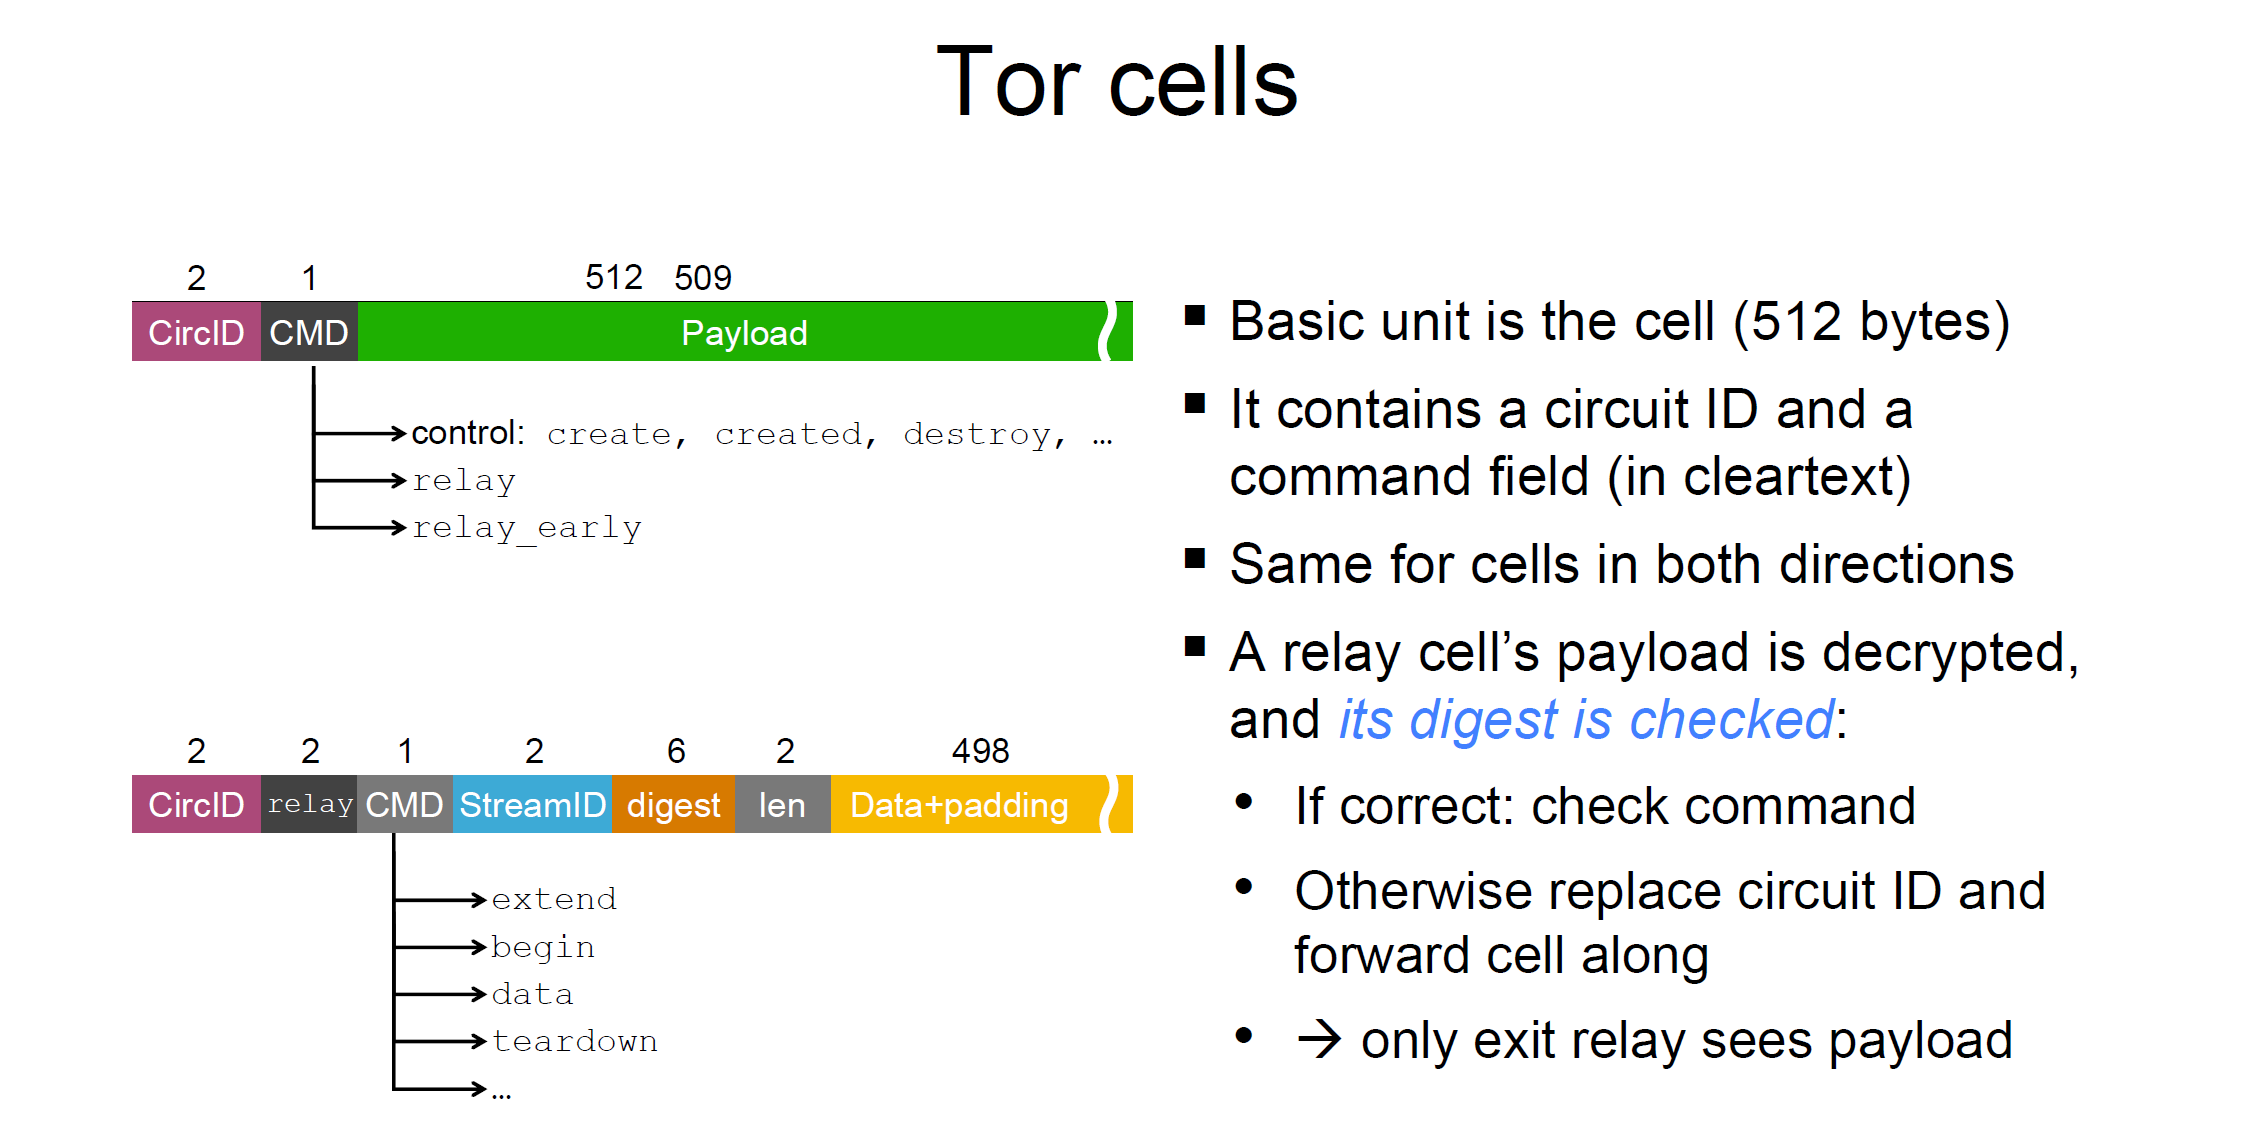
\includegraphics[width=\linewidth]{Figures/Anym_tor_cell.PNG} 
\end{minipage}

\paragraph{Circuit extension with relay\_early:}
\begin{itemize}
    \item Path of arbitrary length can be used for very cheap DoS: Simply create a circuit that goes through all honest nodes, dozens of times: incredibly large amplification factor.
    \item Solution: Tor extend cells can only be contained in relay early cells
\end{itemize}
\\
\textbf{Hidden Services:}\\
\begin{minipage}{\linewidth}
    \centering      
    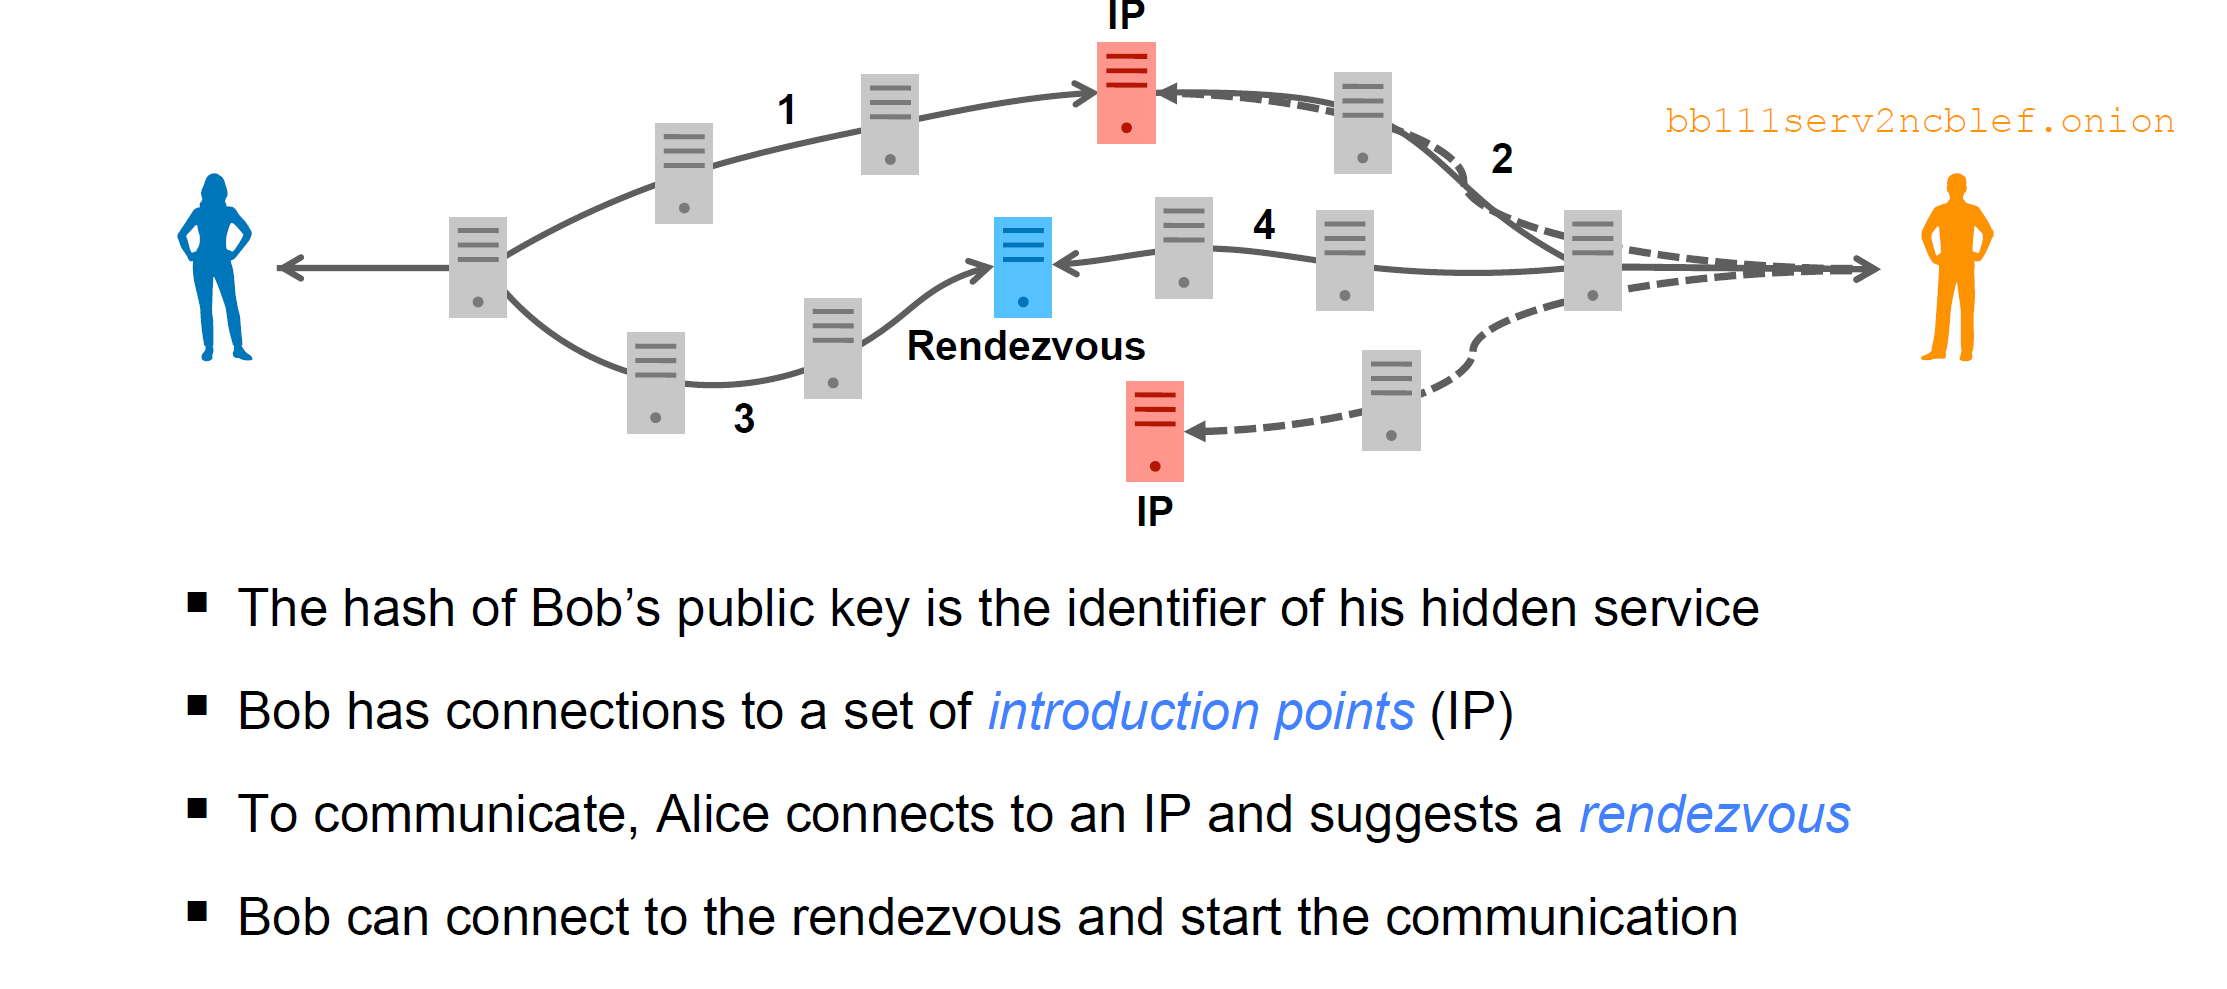
\includegraphics[width=\linewidth]{Figures/Anym_hidden_services.PNG} 
\end{minipage}

\subsubsection{Directory authorities}

\begin{itemize}
    \item How do the clients know what relays there are? 10 directory authorities (servers) running a consensus algorithm.
    \item The authorities track the state of relays, store their public keys.
    \item Client software (Tor browser) comes with a list of the authorities’ keys (If an adversary can supply the list, de-anonymization is trivial!). A client accepts a consensus document if signed by $\geq$ 50\%.
    \item The centralized authorities are an important weakness of Tor. An adversary compromising 5 authorities can compromise Tor.
    \item Every relay periodically reports a signed statement (state, stats.) 
    \item DAs also act as bandwidth authorities: verify bandwidth of nodes.
    \item Sybil protection: DAs limit the number of relays per IP subnet
\end{itemize} 

\subsubsection{Censorship resistance in Tor}
\begin{itemize}
    \item Problem: relay nodes are publicly listed and can be blocked.
    \item The Tor network contains a number of bridge relays (or bridges). Not (all) publicly listed, instead distributed through friends networks. This is used to circumvent censors which black-list Tor relays.
    \item Problem: deep packet inspection allows detection of Tor traffic
    \item Solution: obfuscate the traffic (pluggable transports)
\end{itemize}

\subsubsection{Circuit setup}

Who is authenticated on the first hop? Alice is \textit{not}. The entry guard is since Alice encrypted her ephemeral DH value $g^{x_1}$ with the entry guard's pubKey. The entry guard then sends back $g^{y_1}$ and a hash of $g^{x_1y_1}$ which it can only do if it was able to decrypt $g^{x_1}$ which it can only do if it has the privKey.
\begin{figure}[hb]
	\centering
	\includegraphics[width=0.9\linewidth]{figures/tor_circuit_setup}
	\caption{Circuit setup with three hops}
	\label{fig:torcircuitsetup}
\end{figure}